\chapter{Título da Seção Primária do Desenvolvimento}

\begin{SingleSpace}
\begin{flushright}
\begin{minipage}[b]{8cm}
\begin{small}
``Podem, também, constar epígrafes nas folhas ou páginas de abertura das seções primárias (capítulos)'' (AUTOR, ano, página).
\end{small}
\end{minipage}
\end{flushright}
\end{SingleSpace}

Após o capítulo introdutório, iniciam-se os capítulos do desenvolvimento do estudo. É a parte principal do trabalho, na qual se apresentam a revisão de literatura, os procedimentos metodológicos adotados, a exposição, análise e interpretação dos dados \cite{koche,marconi}.

Divide-se, sistematicamente, em seções e subseções, da primária à quinária, derivadas do tema geral do trabalho \cite{barros}. Todas as seções e subseções devem conter um texto relacionado a elas.

Todo texto deve ser justificado, digitado em fonte \textit{Times New Roman} ou Arial, tamanho 12 e espaçamento de 1,5 entre as linhas, com exceção das citações com mais de três linhas, notas de rodapé, paginação, legendas e fontes das ilustrações e das tabelas, que devem ser em fonte tamanho 10 e espaçamento simples (1,0).

\section{Título da Seção Secundária}

No Brasil, a criação de uma organização nacional de normalização estava voltada ao mercado da construção civil. Em 1940, foi consolidada a Associação Brasileira de Normas Técnicas (ABNT), reconhecida posteriormente, em 1979, como o único Foro Nacional de Normalização.

A ABNT define norma técnica como:

\begin{SingleSpace}
\begin{flushright}
\begin{minipage}[b]{12cm}
\begin{small}
Documento, estabelecido por consenso e aprovado por um organismo reconhecido, que fornece, para um uso comum e repetitivo, regras, diretrizes ou características para atividades ou seus resultados, visando à obtenção de um grau ótimo de ordenação em um dado contexto (ASSOCIAÇÃO BRASILEIRA DE NORMAS TÉCNICAS, 2006, p. 4, grifo do autor).
\end{small}
\end{minipage}
\end{flushright}
\end{SingleSpace}

O uso das normas se tornou um diferencial competitivo para grandes empresas e aos poucos se consolidava a criação de um mercado nacional. A necessidade desses padrões formais é defendida por \citeonline[p. 62]{cunha}:

\begin{SingleSpace}
\begin{flushright}
\begin{minipage}[b]{12cm}
\begin{small}
Todo trabalhador intelectual precisa aceitar a responsabilidade de comunicar adequada e amplamente os resultados de seus estudos e pesquisas, adotando, para tanto, a mesma seriedade, dedicação e disposição de espírito com que encara a responsabilidade de planejar e executar os estudos e as pesquisas que lhe cabem.
\end{small}
\end{minipage}
\end{flushright}
\end{SingleSpace}

Etimologicamente, a palavra conhecimento vem do latim cognoscere e quer dizer vir a saber. Em outras palavras, ``[…] é a relação que se estabelece entre o sujeito que conhece e o objeto que é conhecido'' \cite[p. 5]{cervo}.

Como afirma \citeonline[p. 24]{witter}, ``[…] a sala de aula é um laboratório de pesquisa […]''.

\subsection{Título da seção terciária}

Todas as seções e subseções devem conter um texto relacionado a elas.

\subsubsection{Título da seção quaternária}

As ilustrações - desenhos, esquemas, fluxogramas, fotografias, gráficos, mapas, organogramas, plantas, quadros, retratos, figuras, imagens, entre outros - devem ser inseridas o mais próximo possível do texto a que se referem.

Sua identificação aparece na parte superior, composta pelo nome específico da ilustração, seguido do número de ordem de ocorrência no texto, em algarismos arábicos, travessão e do respectivo título, ajustados às margens da ilustração, em espaço simples (1,0) e alinhamento justificado.

Na Figura 1, apresenta-se a distribuição dos Campi do IFCE pelo estado cearense.

\begin{figure}[!ht]
\Caption{Distribuição dos campi do Instituto Federal de Educação, Ciência e Tecnologia do Ceará}
\centering
\label{campi}
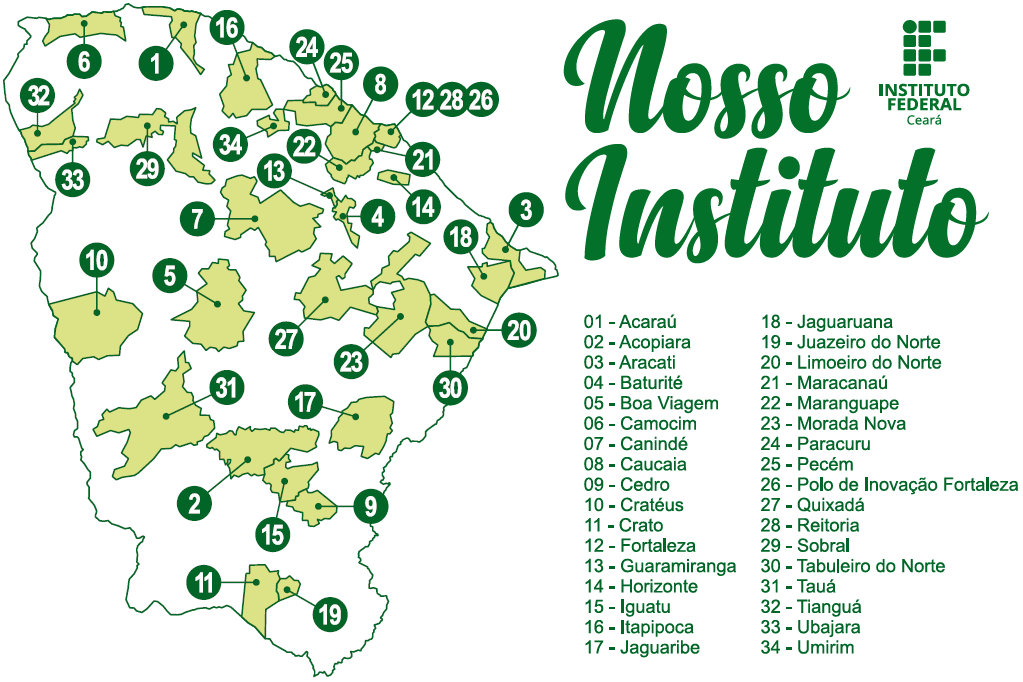
\includegraphics[scale=0.5]{figuras/ifce-estado}
\Fonte{Instituto Federal de Educação, Ciência e Tecnologia do Ceará (2018).}
\end{figure}

\newpage

\subsubsubsection{Título da seção quinária}

As tabelas - apresentação de informações, de forma não discursiva, nas quais o dado numérico se destaca como informação central - devem ser inseridas o mais próximo possível do texto a que se referem.

Sua identificação aparece na parte superior, composta pelo nome tabela, seguido do número de ordem de ocorrência no texto, em algarismos arábicos, travessão e do respectivo título, ajustados às margens da tabela, em espaço simples (1,0) e alinhamento justificado.

\begin{table}[!ht]	
\Caption{Estimativas populacionais brasileiras - Regiões - 2011-2017}
\centering
\label{estimativas}
\begin{tabular}{c|c|c|c|c|c}
\hline
& \multicolumn{5}{c}{\textbf{Regiões}} \\
\cline{2-6}
\textbf{Ano} & \textbf{Sudeste} & \textbf{Nordeste} & \textbf{Sul} & \textbf{Norte} & \textbf{Centro-Oeste} \\
\hline
2011 & 80.975.616 & 53.501.859 & 27.562.433 & 16.095.187 & 14.244.192 \\
\hline
2012 & 81.565.983 & 53.907.144 & 27.708.514 & 16.303.145 &
14.419.229 \\
\hline
2013 & 84.465.570 & 55.794.707 & 28.795.762 & 16.983.484 &
14.993.191 \\
\hline
2014 & 85.115.623 & 56.186.190 & 29.016.114 & 17.231.027 &
15.219.608 \\
\hline
2015 & 85.745.520 & 56.559.481 & 29.230.180 & 17.472.636 &
15.442.232 \\
\hline
2016 & 86.356.952 & 56.915.936 & 29.439.773 & 17.707.783 &
15.660.988 \\
\hline
2017 & 86.949.714 & 57.254.159 & 29.644.948 & 17.936.201 &
15.875.907 \\
\hline
\end{tabular}
\Fonte{Instituto Brasileiro de Geografia e Estatística (2018).}
\end{table}

\begin{flushright}
\begin{minipage}[b]{13.9cm}
\begin{SingleSpace}
\begin{footnotesize}
Notas: Em 2012: \\
\hspace*{0.9cm}
1 - Por determinação judicial e para efeito de distribuição do Fundo de Participação dos Municípios, a população do Município de Brasil Novo-PA é de 17.960 habitantes. Processo Judicial nº 1-28.2012.4.01.3903. \\
\hspace*{0.9cm} 2 - Por determinação judicial e para efeito de distribuição do Fundo de Participação dos Municípios, a população do Município de Jacareacanga-PA é de 41.487 habitantes. Processo Judicial nº 798-41.2011.4.01.3902, Seção Judiciária de Itaituba-PA. \\
\hspace*{0.9cm} Em 2013: \\
\hspace*{0.9cm} Por determinação judicial e para efeito de distribuição do Fundo de Participação dos Municípios, a população do Município de Jacareacanga-PA é de 41.487 habitantes. Processo Judicial nº 798-41.2011 4.01.3902 Seção Judiciária de Itaituba-PA. \\
\hspace*{0.9cm} Em 2014: \\
\hspace*{0.9cm}1 - Por determinação judicial e para efeito de distribuição do Fundo de Participação dos Municípios, a população do Município de Jacareacanga-PA é de 41.487 habitantes. Processo Judicial nº 798-41.2011.4.01.3902, Seção Judiciária de Itaituba-PA. \\
\hspace*{0.9cm} 2 - Por determinação judicial o Município de Coronel João Sá - BA teve os efeitos das estimativas das populações de 2014, 2015 e 2016 suspensas, passando a vigorar, para efeito de distribuição do Fundo de Participação dos Municípios, a população estimada para o ano de 2013, que foi de 17.422 habitantes. Processo Judicial nº 0002222-53.2017.4.01.3306 - Vara Única de Paulo Afonso-BA.
\end{footnotesize}
\end{SingleSpace}
\end{minipage}
\end{flushright}

\newpage

Além do número da população residente, foram extraídas do Portal do IBGE informações populacionais com as variáveis apresentadas no quadro a seguir.

A identificação do quadro aparece na parte superior, composta por seu nome, seguido do número de ordem de ocorrência no texto, em algarismos arábicos, travessão e do respectivo título, ajustados às margens do quadro, em espaço simples (1,0) e alinhamento justificado\footnote{As notas de rodapé têm por finalidade prestar esclarecimentos ou fazer considerações sobre certos aspectos que não devem ser incluídos no texto para não interromper a sequência lógica da leitura.}.

\begin{quadro}[!ht]	
\Caption{Características da população brasileira pesquisadas}
\centering
\label{qua:exemplo-1}
\IFCEqua{}{
\begin{tabular}{|l|l|}
\hline
\textbf{Tema} & \textbf{Variáveis} \\
\hline
Características gerais da população & População residente, situação de domicílio, sexo e idade \\
\hline
Cor ou raça & População residente, idade, sexo, situação de domicílio, educação \\
\hline
Educação & Taxa de alfabetização \\
\hline
Emigração & Emigrantes internacionais \\
\hline
Registro de nascimento & Idade, situação de domicílio, sexo, cor ou raça \\
\hline
Trabalho e rendimento & Idade, sexo, cor ou raça, Índice de Gini \\
\hline
\end{tabular}
}{
\Fonte{Instituto Brasileiro de Geografia e Estatística (2010).}
}
\end{quadro}

\newpage

Para acompanhar o crescimento populacional\footnote{As notas devem constar na mesma página em que ocorre a chamada numérica no texto, digitadas com espaçamento simples (1,0) entre as linhas e alinhadas, a partir da segunda linha da mesma nota, abaixo da primeira letra da primeira palavra, de forma a destacar o expoente, sem espaço entre elas e com fonte tamanho 10.}, anualmente, o IBGE publica estimativas populacionais do nosso país, com dados das regiões, dos estados e, até, dos 5.570 municípios brasileiros\footnote{As notas podem ser de dois tipos: notas de referência e notas explicativas, conforme o Manual de Normalização de Trabalhos Acadêmicos do IFCE.}. 